\documentclass[../../../../../main]{subfiles}
\begin{document}
    \begin{figure}[htbp]
        \centering
        % 1行目
        \begin{subfigure}{.48\linewidth}
            \centering
            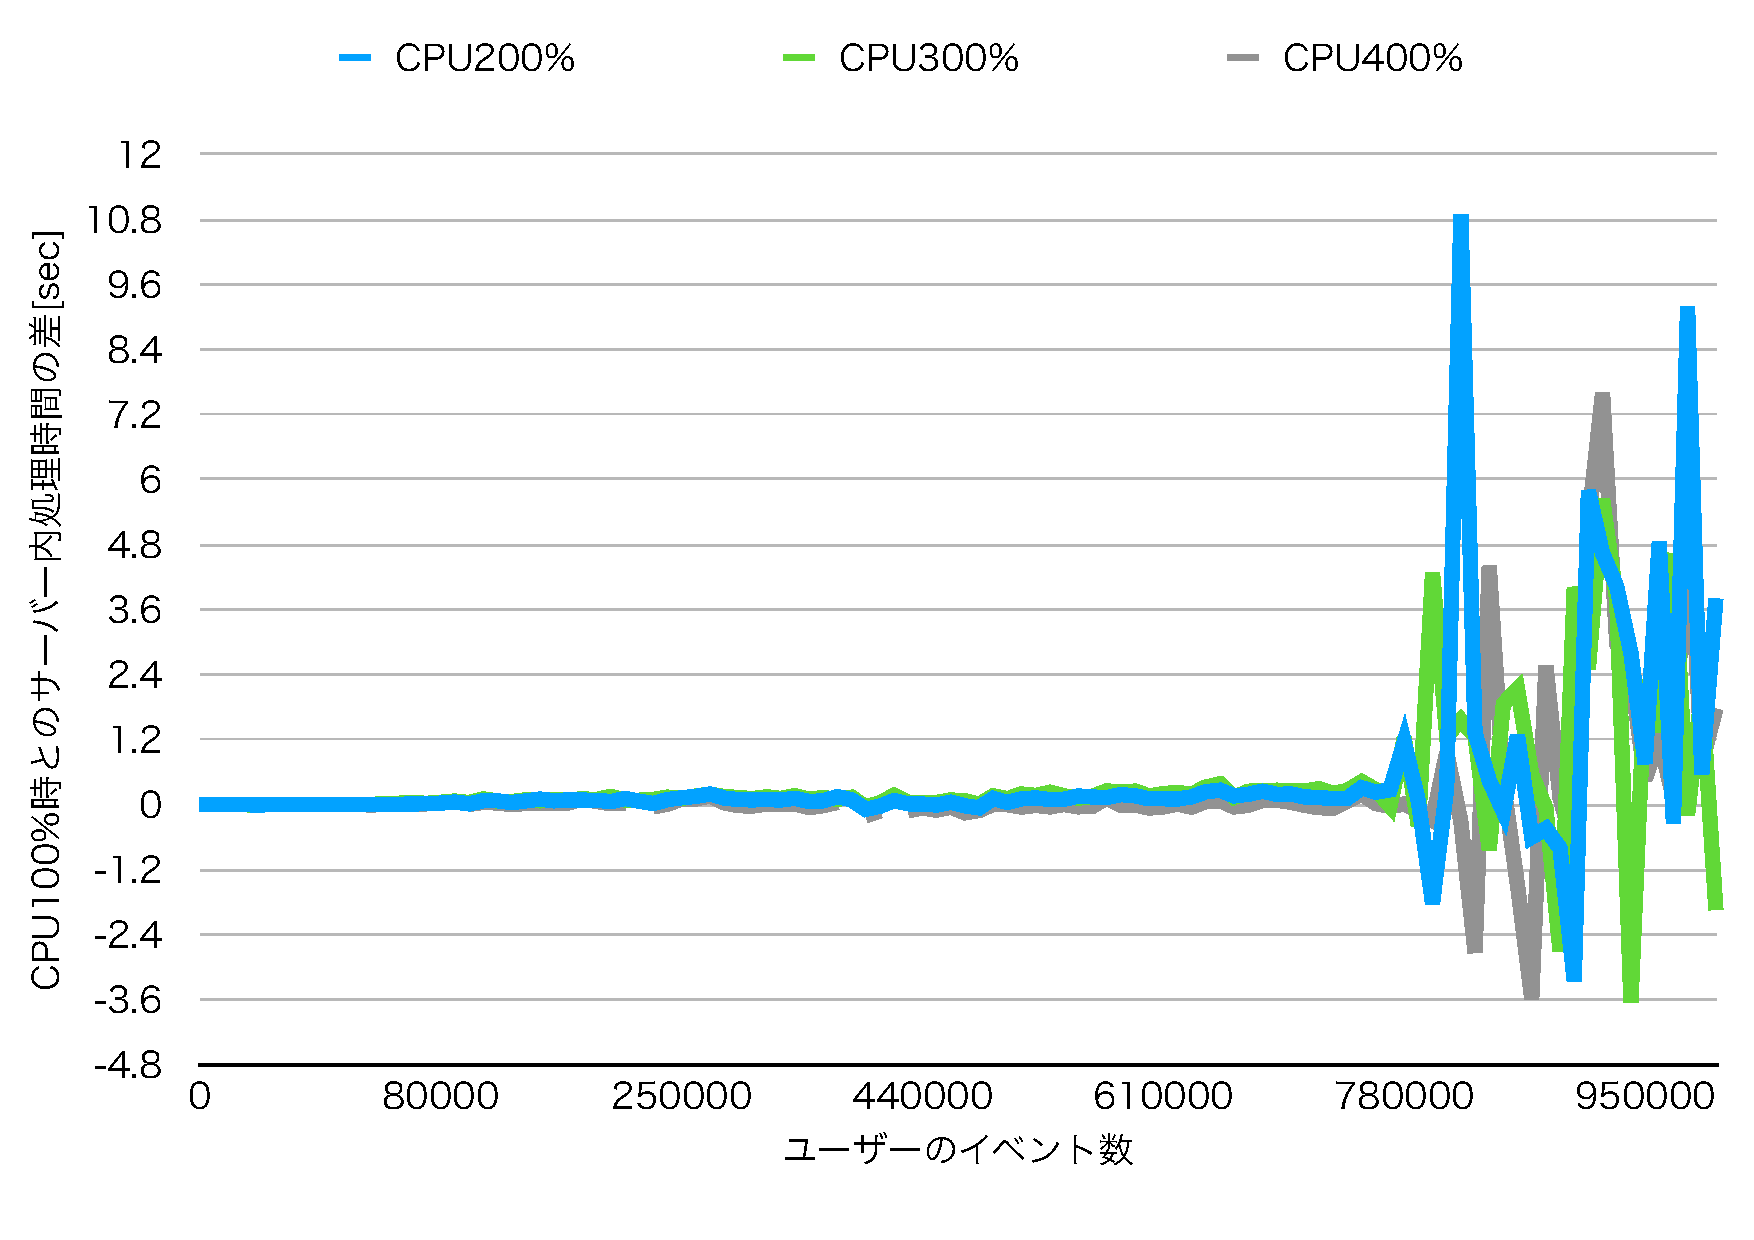
\includegraphics[width=\linewidth]{graph}
            \caption{PDF 1のキャプション}
            \label{fig:pdf1}
        \end{subfigure}\hfill
        \begin{subfigure}{.48\linewidth}
            \centering
            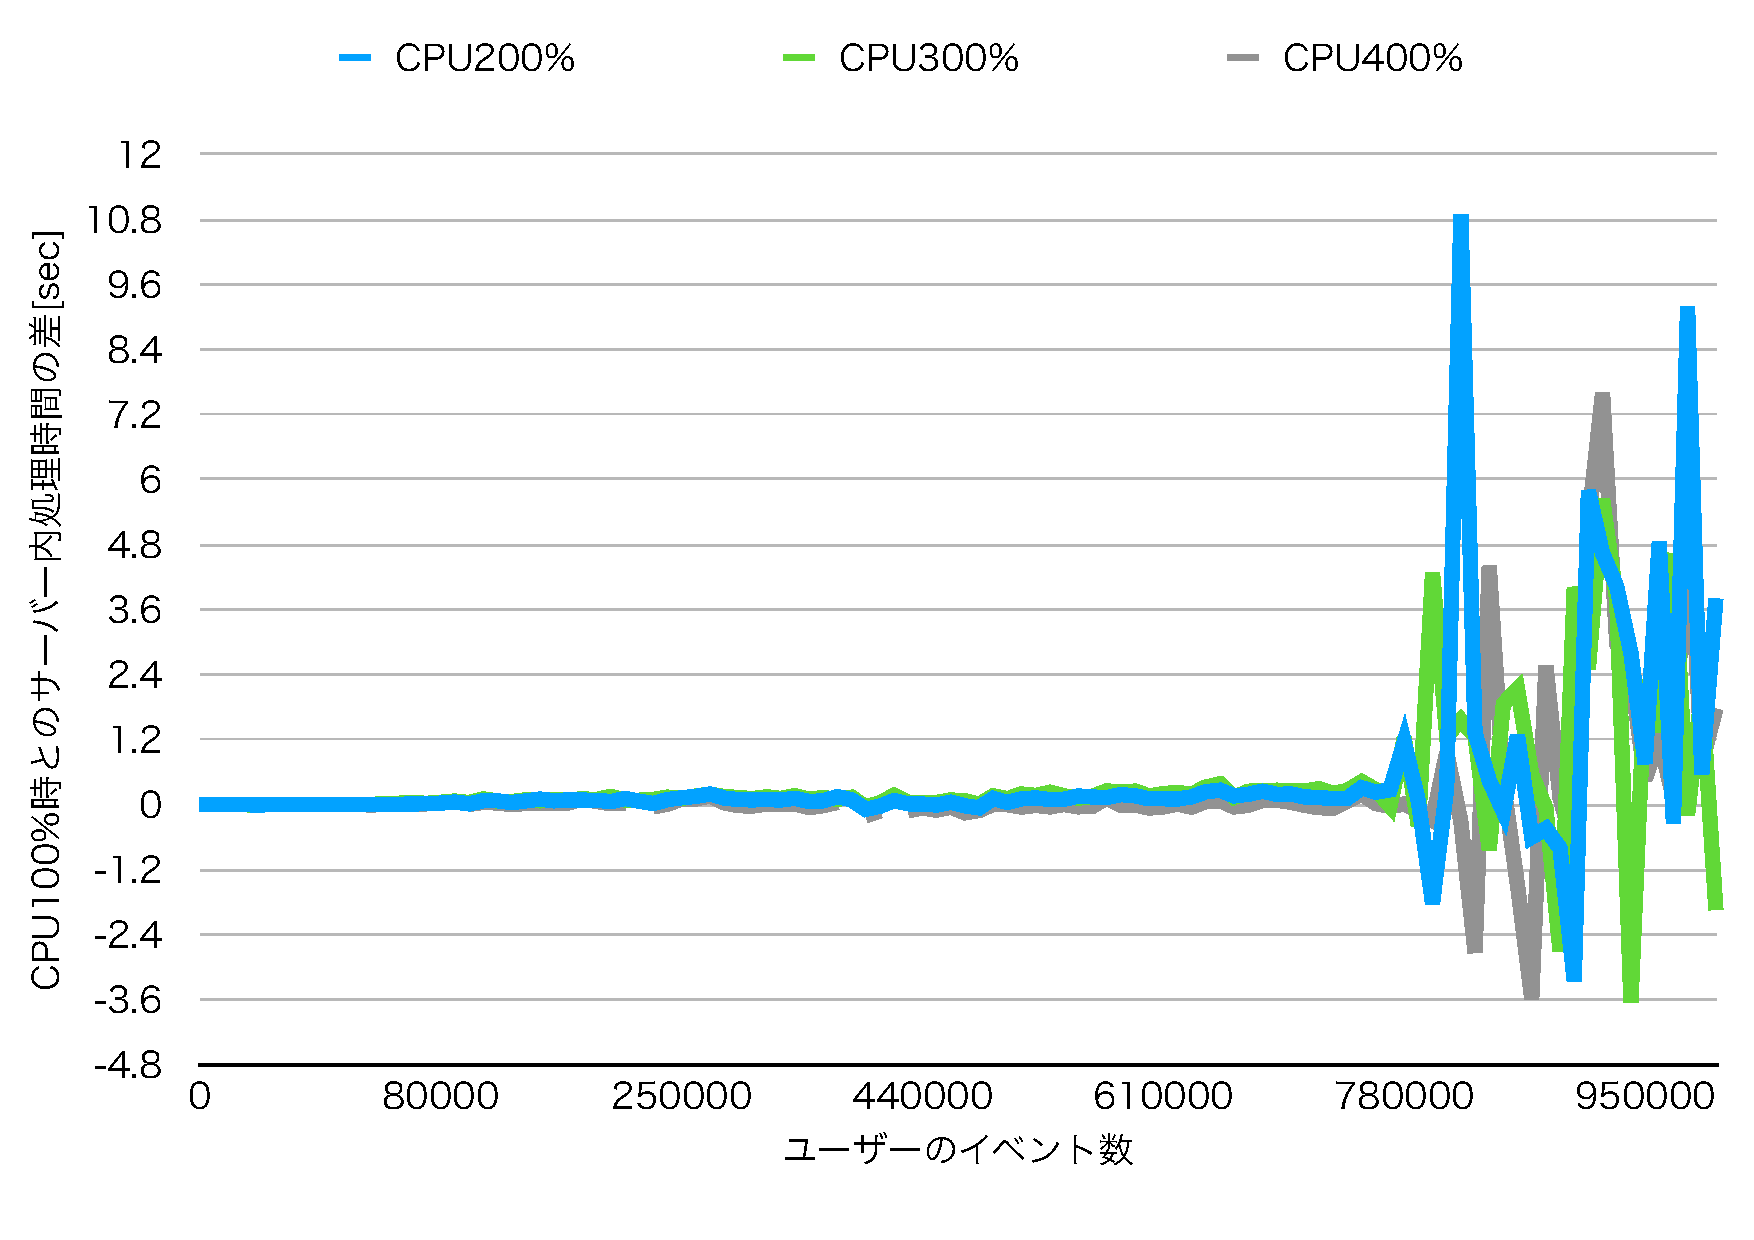
\includegraphics[width=\linewidth]{graph}
            \caption{PDF 2のキャプション}
            \label{fig:pdf2}
        \end{subfigure}

        % 2行目
        \begin{subfigure}{.48\linewidth}
            \centering
            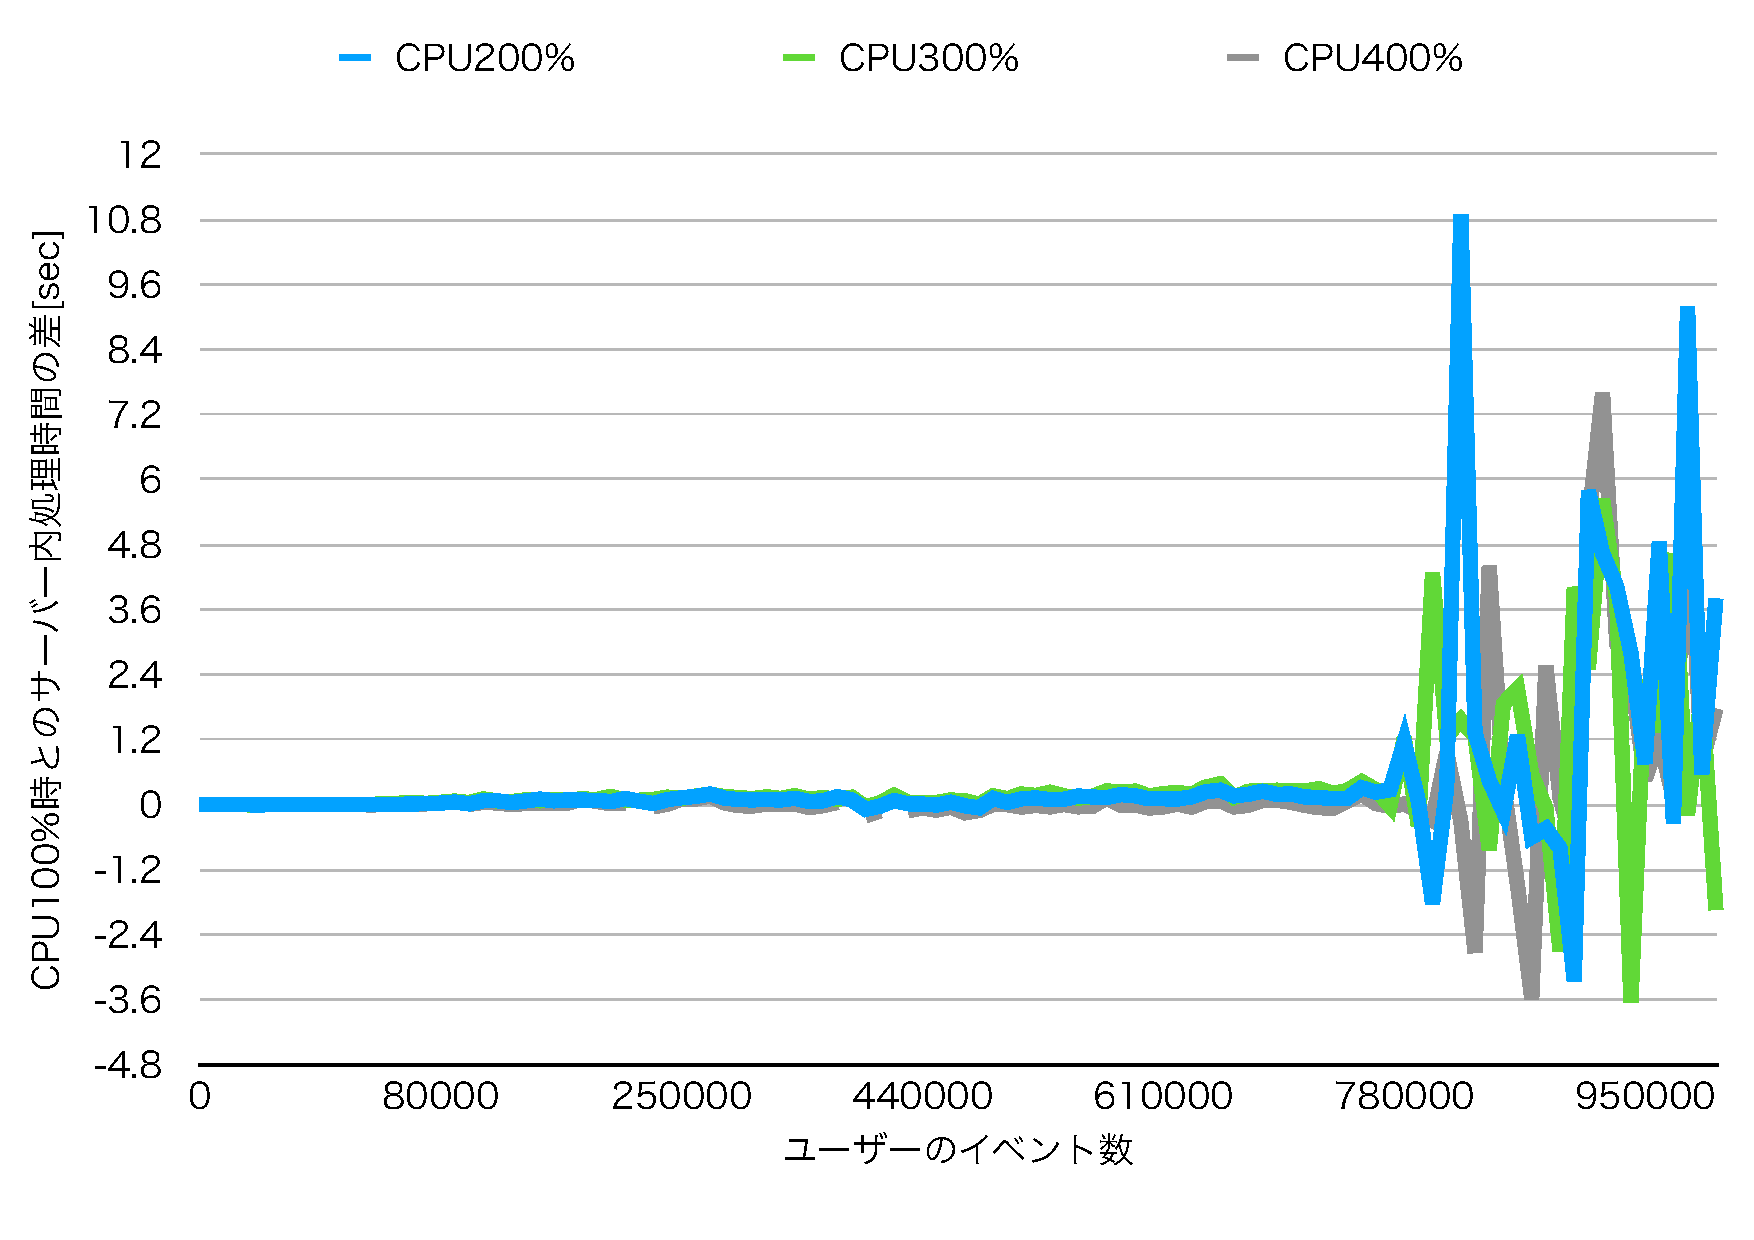
\includegraphics[width=\linewidth]{graph}
            \caption{PDF 3のキャプション}
            \label{fig:pdf3}
        \end{subfigure}\hfill
        \begin{subfigure}{.48\linewidth}
            \centering
            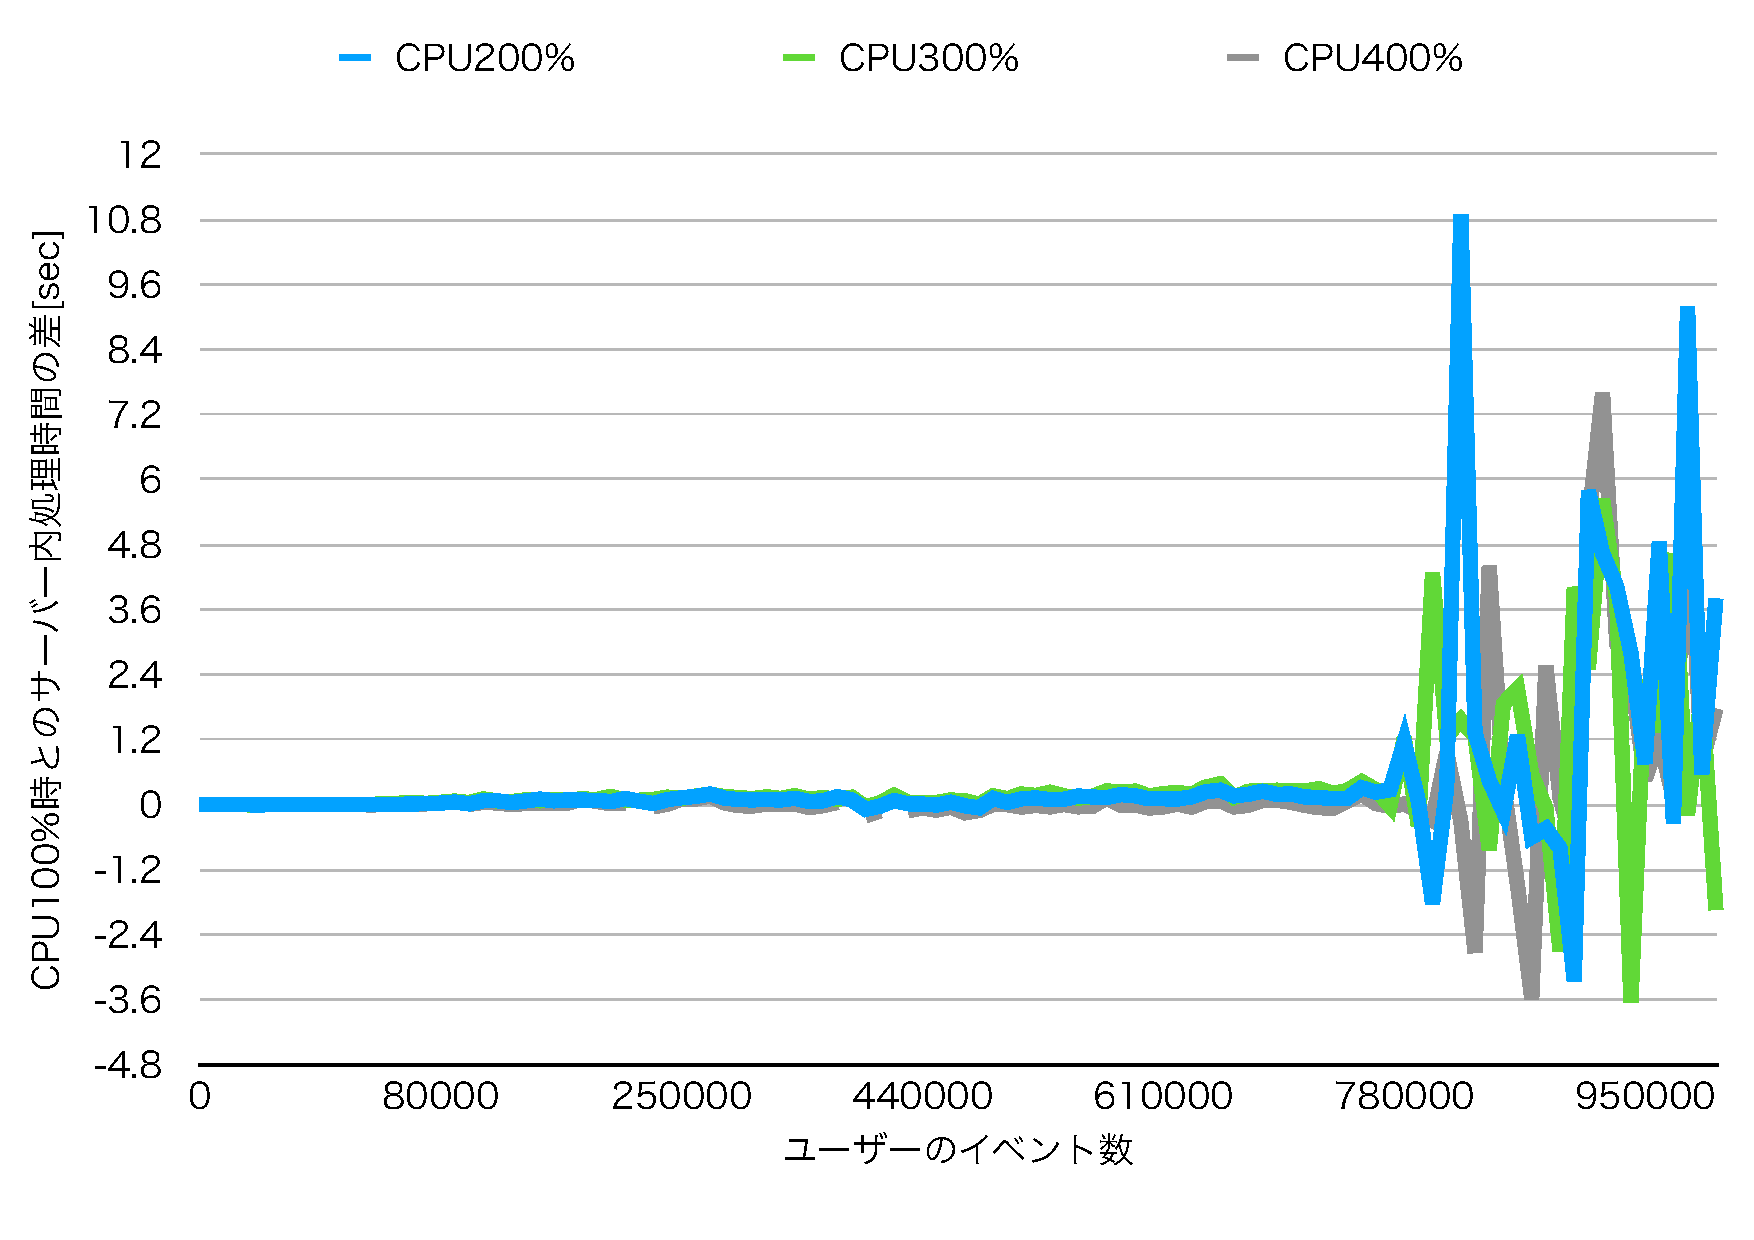
\includegraphics[width=\linewidth]{graph}
            \caption{PDF 4のキャプション}
            \label{fig:pdf4}
        \end{subfigure}
        \caption{全体のキャプション}
        \label{fig:pdfs}
    \end{figure}
\end{document}